\section{Regeln und Regelmengen}
Eine entscheidende Komponente sind Regeln und Regelmengen. Sie werden vom Konfigurator ausgewählt und mit Hilfe des Enumerators ausgeführt.

\subsection{Regelmengen}
Mehrere Regeln werden in einer Regelmenge zusammengefasst.
Insgesamt wurden vier unterschiedliche Regelmenegen implementiert: RS-B0, RS-B1, RS-B2 und GraphRule.
Alle Mengen basieren auf den von Pellenkoft et al. vorgestellten Regelsets.

\begin{figure}[ht]
  \centering
  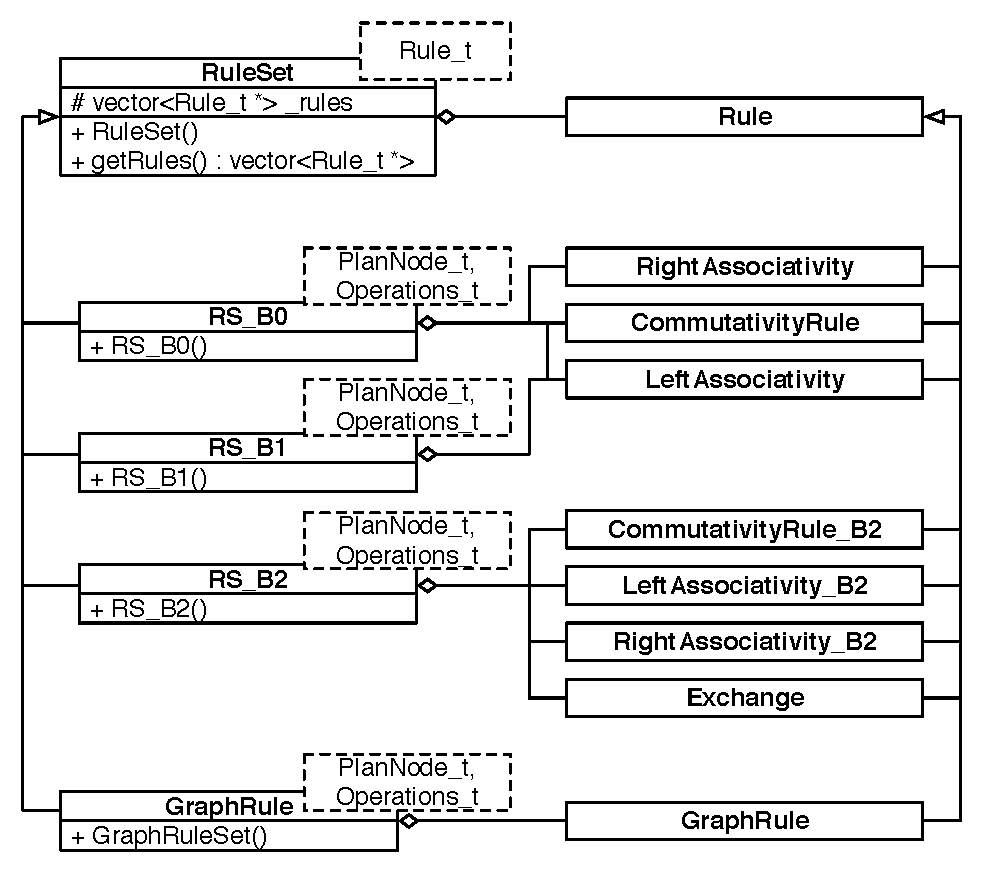
\includegraphics[width=\textwidth]{04_Implementierung/00_media/RuleSets.pdf}
  \caption{Klassendiagramm: Regelmengen und Regeln}
  \label{RuleSetClass}
\end{figure}

\subsubsection{Implementierung}
\label{sec:RuleImplementation}

Alle Regelmengen erben von der Klasse \texttt{RuleSet}, die die Methode \texttt{getRules()} implementiert, mit deren Hilfe ein Vektor von Regeln ausgegeben wird. Je nach Regelmenge können andere Regeln vorhanden sein. Eine Übersicht über Regeln und deren Zuordnung zu Regelsets findet sich in Abb. \ref{RuleSetClass}.

Die einzelnen Regeln bei der Erstellung einer Regelmenge instantiiert und dem Vector \texttt{\_rules} zugeordnet. Die Sammlung der Regeln in einem Vector ist möglich, da alle Regeln von der Abstrakten Klasse \texttt{Rule} erben. 

Konkret ist dem Regelset \texttt{RS-B0} die Regel \texttt{Right Assiciativity}, \texttt{Commutativity} und \texttt{Left Associativity} zugeorndet. Dem Regelset \textit{RS-B1} \textit{Left Associativity} und \textit{Commutativity}. Dem Regelset \textit{RS-B2} sind die Varianten von Kommutativität, Linker und \textit{Rechter Assozativity}, die speziell für diese Regelmenge erstellt wurden zugeordnet ebenso wie die \textit{Exchange} Regel. Der \textit{Graph Rule} wird nur für das \textit{GraphRule Set} benötigt.

\subsubsection{Erweiterbarkeit}
Die Erweiterung der Regelmengen ist in verschiedenen Dimensionen möglich. Neue Funktionen können für die Regelmengen implementiert werden ebenso ist die Erstellung neuer Regelmengen möglich.

Auf Funktionaler Ebene ist es vorstellbar, dass die Reihenfolge der Regeln dynamisiert wird. Aktuell ist es nur möglich, die Regeln in Form eines Vectors auszugeben, dessen Reihenfolge immer gleich ist. Da alle konkreten Regelmengen von der selben Klasse \texttt{RuleSet} erben, ist die Implementierung einer anpassbaren Reihenfolge leicht möglich und muss für alle Klassen nur einmal vorgenommen werden.


Auch das Hinzufügen von neuen Regeln zu bestehender Regelmengen oder die Erweiterung von bestehenden Regelmengen ist möglich. Beispielsweise kann von bestehenden Regelmengen geerbt wird bzw. neue Regeln und deren Regelmengen durch die Implementierung der standardisierten Interfaces \texttt{RuleSet} entstehen.

Die Erweiterbarkeit konnte mit der Implementierung der Regelmenge  \textit{Graph Rule} unter Beweis gestellt werden, da diese Regelmenge erst später entwickelt wurde und auf die bestehende Infrastruktur aufsetzte.




\subsection{Regeln}

\begin{figure}[ht]
  \centering
  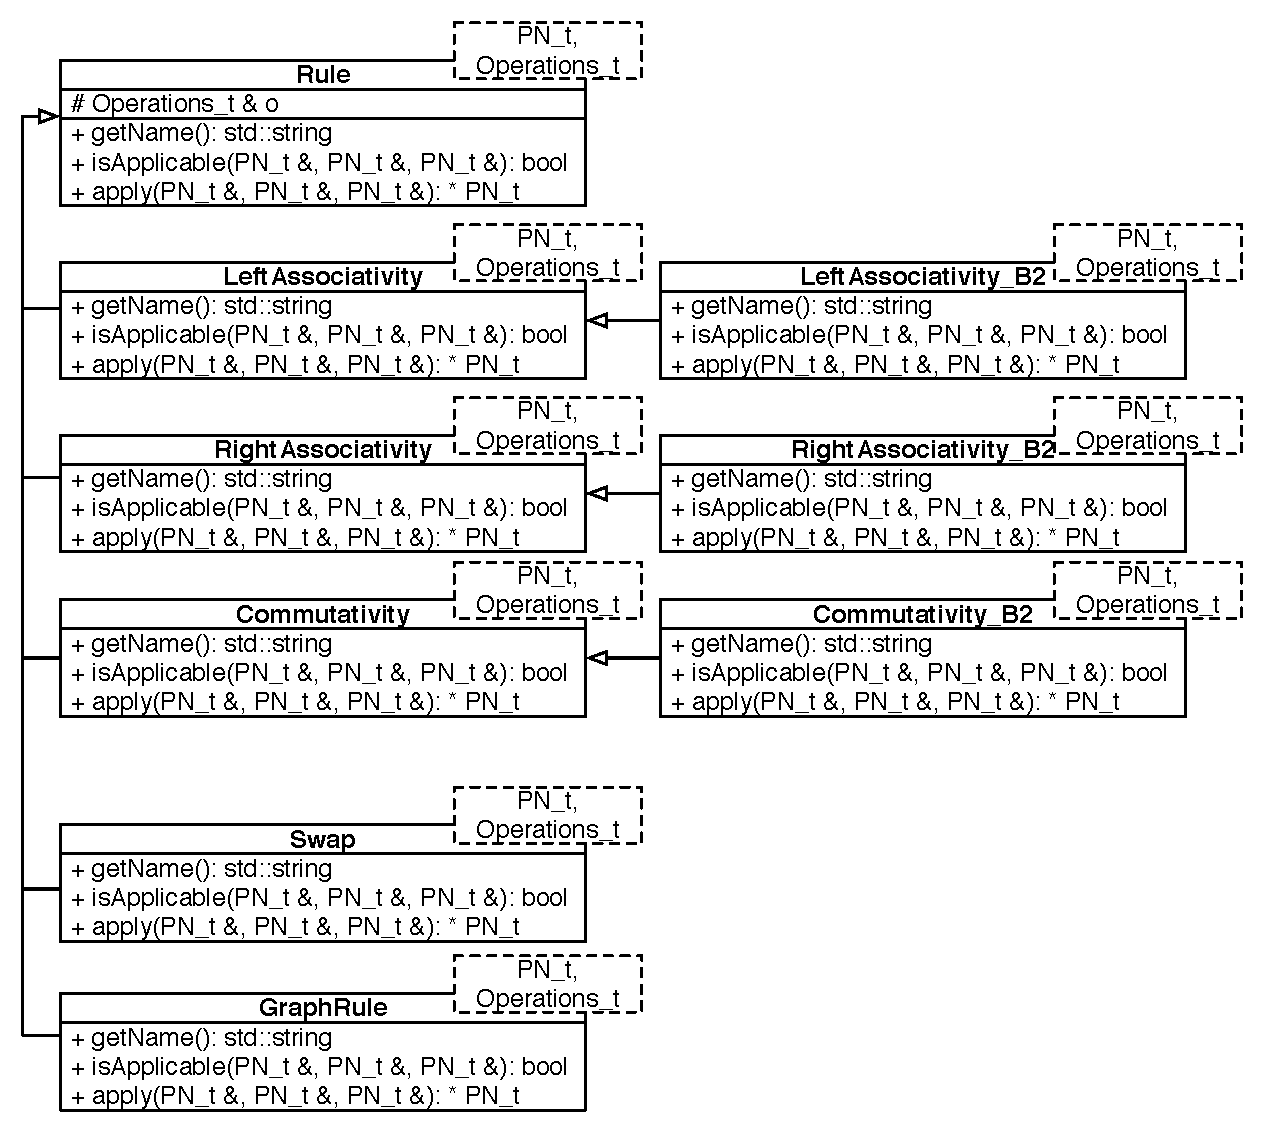
\includegraphics[height=\textwidth]{04_Implementierung/00_media/Rules.pdf}
  \caption{Klassendiagramm: Regeln}
  \label{RuleClassDiagram}
\end{figure}

Die einzelnen Regeln, die Teil der Regelmengen sind, werden jeweils in einer eignen Klasse abgelegt. Aktuell sind acht Regeln vorhanden: (1) \texttt{Commutativity}, (2) \texttt{Left Associativity}, (3) \texttt{Right Associativity}, (4) \texttt{Commutativity B2}, (5) \texttt{Left Associtativity B2}, (6) \texttt{Right Associativity B2}, (7) \texttt{Exchange}, (8) \texttt{Graph Rule}. Die Zuordnung der Regeln zu den unterschiedlichen Regelmenegen wurde in \ref{sec:RuleImplementation} erklärt und in Abb. \ref{RuleSetClass} veranschaulicht.

\subsubsection{Implemenetierung}


Auch bei den Regeln erben alle Regeln direkt oder - und das ist neu - indirekt von der Klasse \texttt{Rule}. Die Organisation der Klassen ist in Abb. \ref{RuleClassDiagram} dargestellt. Alle Regeln Implementieren das Interface, das durch die Abstrakte Klasse \texttt{Rule} vorgegeben ist. Durch die Methode \texttt{getName()} wird der Name der jeweiligen Regel zurückgeliefert. Wie bei anderen Implementierungen sind die Regeln in zwei Teilen organisiert. Mit Hilfe der Methode \texttt{isApplicable} kann festgestellt werden, ob eine Regel anwendbar ist, Die Methode \texttt{apply} wendet die Regel an und liefert einen Plan-Knoten zurück. Der Plan-Knoten selbst sowie die Operationen, die zur Erzeugung eines neuen Plans führen können durch Template Parameter ausgetauscht werden. So ist es möglich andere Plan-Knoten zu verwenden und die Funktionsweise von Operationen wie \texttt{JOIN} völlig neu zu bestimmen.


Die konkrete Implementierung der Regeln lässt sich am besten am beispeil eines konkreten Plans erläutern. ein solcher konkreter Plan ist in Abb. \ref{SimplePlan} zu sehen. Der oberte Knoten wird als \textit{parent} bezeichnet. Der linke untergeordnete Knoten als \textit{left} und dessen linker Knoten als \textit{left.left}. Analog dazu sind die Bezeichnungen der anderen Knoten gewählt. 

\begin{figure}[ht]
  \centering
  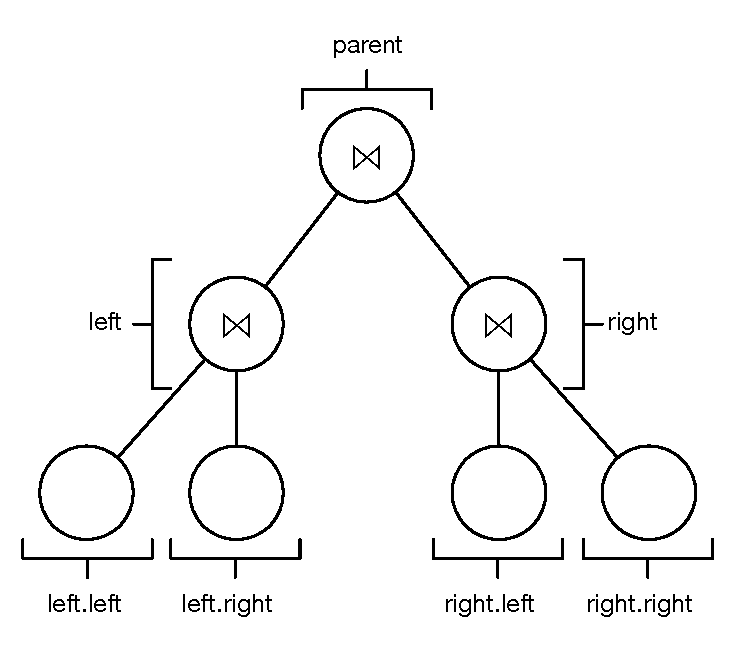
\includegraphics{04_Implementierung/00_media/Plan.pdf}
  \caption{Plandiagramm: Einfacher Beispiel-Plan}
  \label{SimplePlan}
\end{figure}

Auch Join-Kanten sind für die Knoten gegeben und in Abbildung \ref{JoinEdgeMap} abzulesen. Für jeden Knoten sind des Join-Kanten-Nachbarn eingetragen.
